\scanpage{339}

À tout $X_*\in\operatorname{Ob}\widehat\Delta=\operatorname{Ob}S_s$,
on associe le foncteur
\[
F_{X_*}:M_*\longmapsto\operatorname{Hom}_{\widehat\Delta}(X_*,M_*)
\simeq\operatorname{Hom}_{\widehat\Delta_{k\text{-ab}}}
(\underbrace{k[X_*]}_{\Vert},M_*)\in\mathrm{Ab}_k
\]
\[
(F_{X_*}\in\underline{\operatorname{Hom}}_{k\text{-add}}(\mathrm{Ab}_*,\mathrm{Ab}_k))
\quad\unsure{\ni|\in}G_{(\lambda_*)}(M_*)
\]
\[
\Vert\quad G_{\lambda_\bullet}(M_\bullet)
\]
\margin{\[
\lambda_*=C_*(X_*)
\]
\[
\Vert\quad n\longmapsto C_{[n]}(X_*)=k[X_{[n]}]=k^{(X_{[n]})}
\]}

La donnée d'un tel foncteur $F$ \inserted{$k$-add}
équivaut à la connaissance de $F(C_*^\bullet)\in\mathrm{Ab}_k^\bullet$.
\[
F(C_*^\bullet)=(i\longmapsto F(C_*^i))\in\mathrm{Ab}_k
\]

On a
\[
F_{X_*}(C_*^i)\simeq C^i(X_*)\subset k^{X_{[i]}}
\quad(\text{cochaines \uline{non dég}})
\]
\[
\rotatebox{90}{$\simeq$}\qquad C_i(X_*)^\vee
\]
\margin{\figure{\begin{tikzpicture}\node[draw,ellipse] {Plus gén, $G_{\lambda_*}(C_*^\bullet)\simeq\lambda_\bullet^\vee$};\end{tikzpicture}}
\[
\Vert\quad G_{\lambda_\bullet}(C_\bullet^\bullet)
\]}
\[
F_{X_*}(C_*^\bullet)\simeq C^\bullet(X_*)
=\text{complexe}\ \text{des cochaines non dégénérées sur }X_*
\]

\uline{Ex}
\[
X_* =\Delta_*^n,\qquad
\left\{\begin{aligned}
F_{\Delta_*^n}(M_*)&\simeq M_{[n]}\\
C^\bullet(\Delta^n)&\simeq(C_{[n]}^i)_i
=\Lambda^{*+1}k^{\Delta^n}
=(m\longmapsto k^{\operatorname{Mon}(\Delta_*^m,\Delta_*^n)})
\end{aligned}\right.
\]

On s'intéresse, pour $X_*$ fixé, à
\[
[n]\longmapsto\operatorname{Hom}(F_{X_*},F_{\Delta_*^n})
\simeq\operatorname{Hom}(\underbrace{C^\bullet(X_*)}_{\substack{\Vert\\\lambda_\bullet^\vee}},
\underbrace{C^\bullet(\Delta_*^n)}_{\substack{\Vert\\\Lambda^{\bullet+1}k^{\Delta^n}=C_{[n]}^\bullet}})
\]
\diagram{\begin{tikzcd}[column sep=large,row sep=large]
& {} &\\
&\deleted{\operatorname{Hom}(G_{\lambda_*},G_{C_*(\Delta^n)})}
\arrow[u,no head,"\rotatebox{90}{$\simeq$}"'] &\\
k[X_n]\arrow[uur,bend left=25] &
\operatorname{Hom}(\Delta^n,X_*)=X_n \arrow[l] \arrow[uu] &
\end{tikzcd}}
\[
u\longmapsto F(u)\qquad
\lambda_*=C_*[X]\qquad \Vert\ \mu_*
\]
\figure{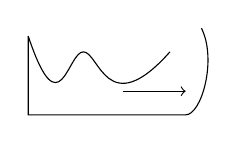
\begin{tikzpicture}
\draw (0,1) -- (0,0) -- (2,0) .. controls (2.2,0) and (2.4,.7) .. (2.2,1.1);
\draw (0,1) .. controls (.4,-.2) and (.5,.8) .. (.7,.8)
.. controls (.9,.8) and (1,-.1) .. (1.8,.8);
\draw[->] (1.2,.3) -- (2,.3);
\end{tikzpicture}}
\diagram{\begin{tikzcd}
\deleted{K} & \deleted{\mathrm{Ab}_{k*}}\arrow[l,shift left] \arrow[l,shift right,no head]
\arrow[dr,no head] &\\
&&\deleted{\unsure{\operatorname{Hom}}}
\end{tikzcd}}

\margin{\[
\rotatebox{90}{$\simeq$}\qquad\operatorname{Hom}(C_\bullet^{[n]},\lambda_\bullet^{\vee\vee})
\]
\[
\rotatebox{90}{$\simeq$}\,!\qquad(\lambda_\bullet^{\vee\vee})_{[n]}=\lambda_{[n]}^{\vee\vee}
\]
\[
\Vert\qquad k[X_{[n]}]^{\vee\vee}
\]}

R. Ainsi \unsure{on a} diagramme comm.

\margin{\[
\deleted{\unsure{\operatorname{Hom}(C_\bullet(X_*)^{\vee\vee},\Lambda^{\bullet+1}k^{\Delta^n})}}
\]
\[
\operatorname{Hom}_\bullet(\Lambda^{\bullet+1}k^{\Delta^n},C_\bullet(X_*)^{\vee\vee})
\]
\[
\rotatebox{90}{$\simeq$}\qquad\operatorname{Hom}(C^\bullet(X_*),\Lambda^{\bullet+1}k^{\Delta^n})
\]
\[
\rotatebox{90}{$\simeq$}
\]}
\figure{\begin{tikzpicture}\draw (.5,1.4) .. controls (-.4,-.2) and (0,-.8) .. (.5,-.8) -- (1.6,-.8);\end{tikzpicture}}

\diagram{\begin{tikzcd}[column sep=large,row sep=large]
X_{[n]}\arrow[d] & \operatorname{Hom}(\Delta_*^n,X_*)\arrow[dd] \arrow[l,"\simeq" description,no head]\\
k[X_{[n]}]\arrow[d,"(\text{iso si }X_n\text{ fini})"'] &\\
k[X_{[n]}]^{\vee\vee} &
\operatorname{Hom}(F\deleted{(X_*}_{\inserted{X_*}},F_{\Delta_*^n})\simeq\operatorname{Hom}(C^\bullet(X_*),C^\bullet(\Delta_*^n))
\arrow[l,"\sim"]
\end{tikzcd}}

Faisons en particulier $X_*=\Delta_*^m$, on trouve donc
\diagram{\begin{tikzcd}[column sep=large,row sep=large]
\Delta_{[n]}^m=\operatorname{Hom}(\Delta^n,\Delta^m)\arrow[d]
\arrow[r,"\simeq" description,no head] & \operatorname{Hom}(\Delta_*^n,\Delta_*^m)\arrow[d]\\
k(\Delta_{[n]}^m)\arrow[r,"\simeq" description,no head] &
\operatorname{Hom}(F_{\Delta_*^m},F_{\Delta_*^n})\simeq
\end{tikzcd}}

\mspage{340}
